\chapter{Fundamentos Teóricos de hornos}
\par En este capítulo se presenta un resumen de los conceptos teóricos, modelos matemáticos y algoritmos necesarios para comprender el desarrollo del trabajo y realizar los cálculos que se usaran luego en la sección de metodología.
\par En primer lugar se da una definición de horno de proceso, se explican los tipos de hornos y las secciones generales que componen estos hornos. Luego se describen los métodos de resolución de ecuaciones utilizados. Por último, se elabora sobre las ecuaciones necesarias para simular los fenómenos en cada sección del horno.

\section{Hornos de fuego directo}
\par Un horno se define como un equipo cerrado dentro del cual se transfiere calor a cualquier tipo de cuerpo y/o sustancia. Éstos presentan distintas formas y modos de transferencia de calor, dependiendo de la sustancia que se va a introducir en el equipo y el tipo de servicio que va a prestar. Funciona como un intercambiador de calor en el que el fluido que transfiere calor al fluido del proceso son gases de combustión que contienen una alta energía térmica, debido a la generación de una gran cantidad de calor en el proceso de combustión, por los altos valores del poder calorífico de los combustibles.\cite{bib:biset}

\subsection{Usos principales de los hornos en refinerías de petróleo}
\par La utilización de estos equipos puede tener distintos propósitos como precalentamiento de una corriente previo a su fraccionamiento o reacción, evaporar la corriente de fondo de una columna de destilación o disminuir la viscosidad de un fluido para facilitar su manipuleo.
Pueden utilizarse también como reactores, en este caso proveen el calor de reacción. La cantidad de combustible alimentado al horno se regula normalmente en función de la temperatura de salida de la corriente de proceso.
\par Los hornos son definidos en función de su capacidad de suministro de calor (Duty), medida en millones de Kcal/h o en millones de Btu/h. Para la mayoría de los hornos instalados en la industria petrolera, la capacidad suele oscilar entre 10 y 350 MM de Btu/h.

\subsection{El horno como un intercambiador de calor}
\par Pueden ser considerados intercambiadores de calor a contracorriente, en los que el fluido de proceso fluye dentro de tubos y se calienta por radiación procedente de una llama de combustión y por convección desde los gases calientes de esta.

\subsection{Clasificaciones de los hornos}
\par Los hornos suministran calor a un fluido de proceso por radiación y convección a partir de la circulación de los gases calientes producto de la combustión dentro de la cámara de combustión, donde el conjunto de tubos que contienen el fluido de proceso pueden estar dispuestos de distintas maneras.\cite{bib:sandoval}
\par Los hornos son clasificados dependiendo de su diseño mecánico, como se puede apreciar en la Figura \ref{fig:hornos_tipos} las seis clasificaciones b\'asicas son las siguientes:\cite{pdvsa1}
\begin{enumerate}[label=\Alph*]
    \item .-  Hornos tipo cilíndrico con serpentines verticales.
    \item .-  Hornos tipo cilíndrico con serpentín helicoidal.
    \item .-  Hornos tipo cabina doble con serpentines verticales.
    \item .-  Hornos tipo cabina con serpentín horizontal.
    \item .-  Hornos tipo cabina con serpentín albor.
    \item .-  Hornos tipo cabina doble con serpentines horizontales.
\end{enumerate}
\begin{figure}[hbt]
\begin{center}
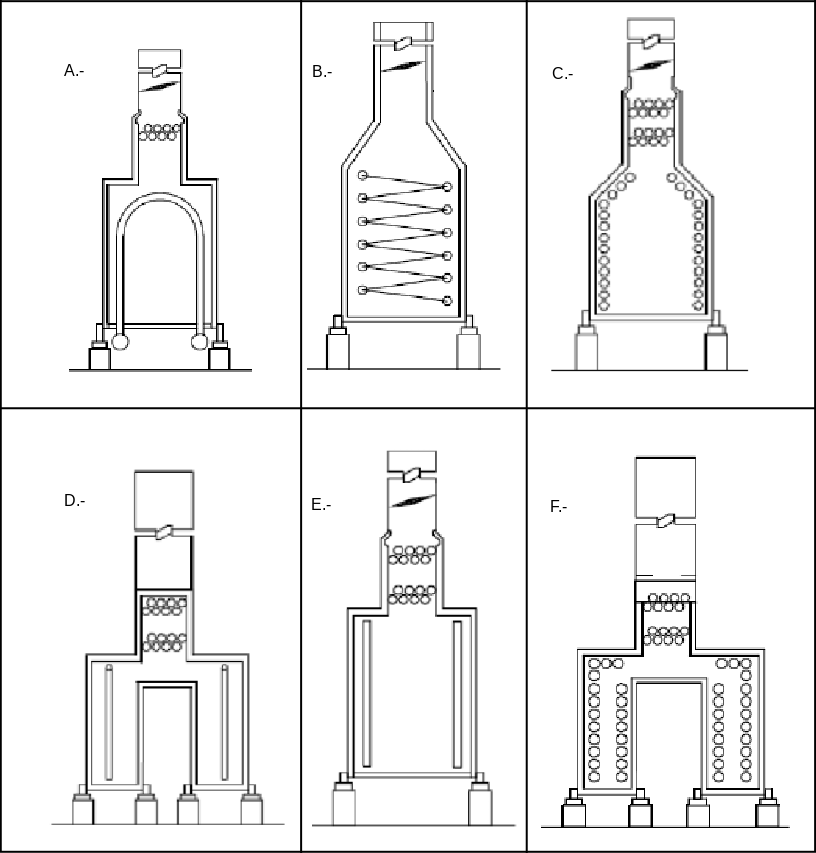
\includegraphics[scale=0.30]{images/hornos_tipos}
\caption[Tipos de hornos por diseño mecánico]{Clasificación de de hornos según su diseño mecánico.\cite{kumar}}
\label{fig:hornos_tipos}
\end{center}
\end{figure}

\subsubsection{Disposición de los quemadores}
\par La ubicación de instalación y la orientación de los quemadores se conoce como disposición de los quemadores.
\par Los quemadores se pueden instalar en el piso, las paredes o el techo de la sección radiante y se pueden colocar para encenderlos hacia arriba, hacia los lados o hacia abajo. Los quemadores montados en la pared, encendidos horizontalmente, se describen además como encendidos en la pared de fondo o en la pared lateral.\cite{kumar} Los quemadores de la pared de fondo se encienden horizontalmente a lo largo de la sección radiante. Los quemadores de pared lateral dirigen las llamas a lo ancho de la sección radiante. (ver Figura \ref{fig:quemadores})
\begin{figure}[hbt]
\begin{center}
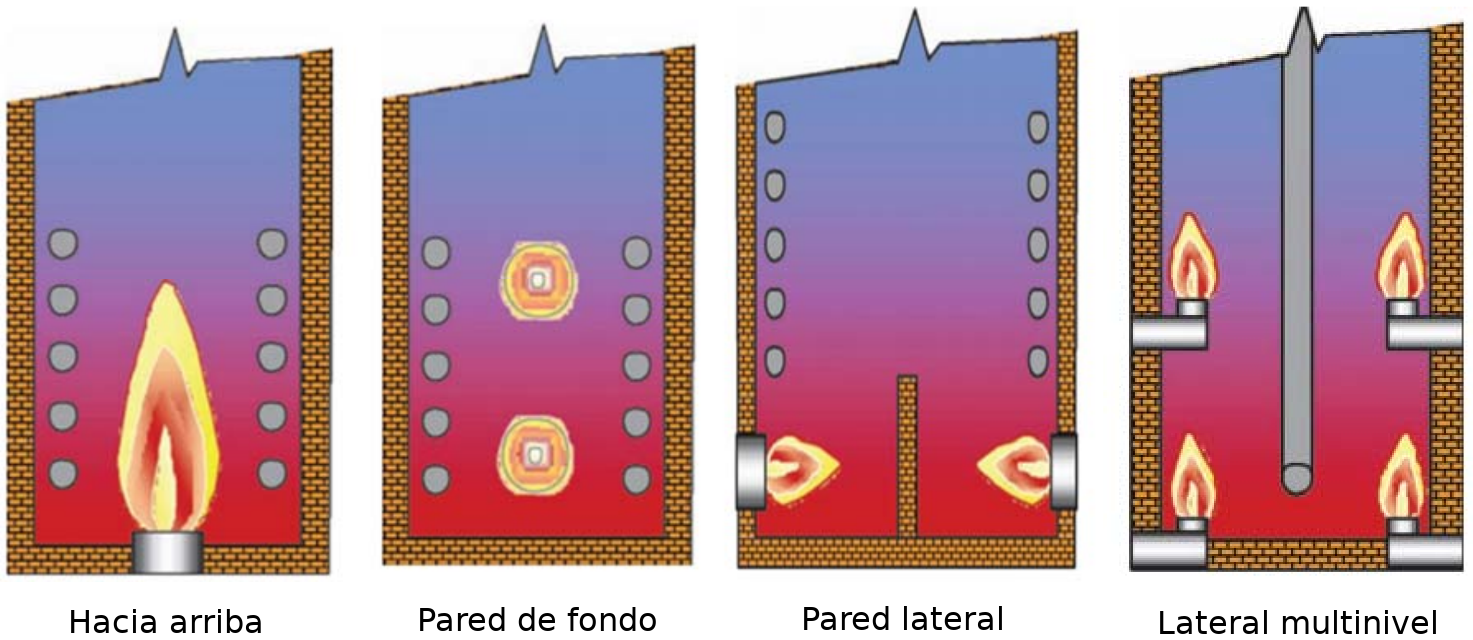
\includegraphics[scale=0.30]{images/quemadores}
\caption[Disposición de los quemadores]{Disposición de los quemadores.\cite{kumar}}
\label{fig:quemadores}
\end{center}
\end{figure}

\subsubsection{Tiro}
\par Es la presión negativa (vacío) en un punto dado dentro del horno, expresado usualmente en kPa (pulgadas de agua), existen tres clasificaciones de tiro para los distintos hornos.
\begin{enumerate}[]
    \item Tiro natural: es el sistema mediante el cual el tiro requerido para llevar el aire de combustión dentro del horno y extraer los gases de combustión del mismo es suministrado solamente por la chimenea.
    \item Tiro forzado: el uso de un ventilador de tiro forzado se requiere para suplir el aire de combustión a los quemadores y para vencer la caída de presión a través de los quemadores. Esto es contrario al tiro natural, donde la columna de gases caliente en la chimenea y el horno proveen la succión para atraer el aire para combustión al horno.
    \item Tiro inducido: se usa un ventilador en el lado del flujo de gases de combustión del horno, para proveer el tiro adicional requerido (mayor que el suplido por la chimenea), para sacar el gas de escape a través de la sección de convección.
\end{enumerate}

\par El horno escogido para simular en este proyecto ha sido uno de tipo cabina con serpentín horizontal de tiro natural, descrito en la Figura \ref{fig:diagrama-meca}, tomando de referencia el horno de una unidad de destilación al vació ubicada en una refinería de Venezuela.

\begin{figure}[hbt]
\begin{center}
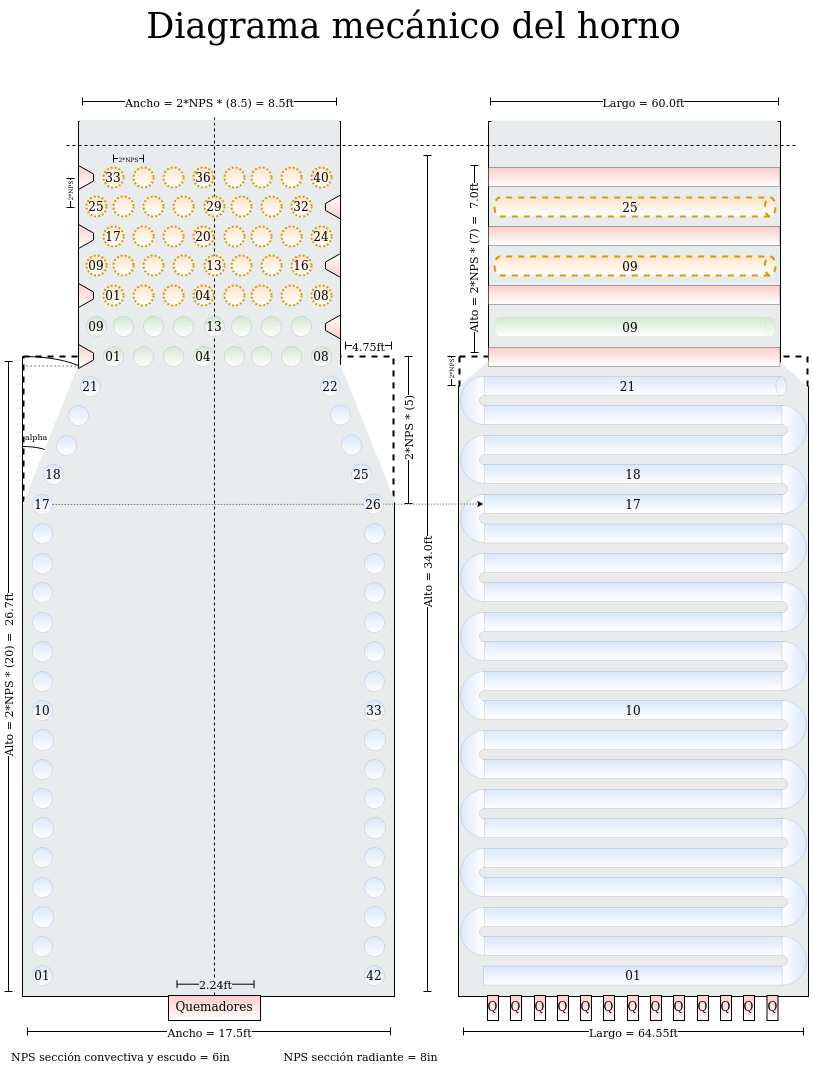
\includegraphics[scale=0.38]{images/diagrama-meca}
\caption[Diagrama mecánico]{Diagrama mecánico del horno simulado.}
\label{fig:diagrama-meca}
\end{center}
\end{figure}

\subsection{Secciones y componentes del horno}
\subsubsection{Sección radiante (hogar)}
\par En esta zona los tubos que contienen el fluido de proceso se encuentran directamente con la llama de combustión, por lo que el calor transferido se debe en un 80\% por radiación y un 20\% por convección. 
\par \textbf{Cámara de combustión}: es el término usado para describir la estructura que circunda los serpentines radiantes y dentro de la cual se localizan los quemadores.
\par \textbf{Los quemadores}: se encargan de la preparación final del combustible y de su combustión. La preparación del combustible consta de su mezcla con aire para luego atomizarlo y vaporizarlo para su posterior combustión. Representan la principal fuente de energía para el movimiento y quema de los gases y por ende son la principal fuente de calor del horno, se pueden ubicar en diferentes zonas de la cámara de combustión, pueden ser de piso, techo, laterales o pared.
\par \textbf{El serpentín}: es el componente más importante y más costoso a la hora de la instalación de un horno, es en él donde se produce la transferencia de calor y debe seleccionarse tomando en cuenta la temperatura, el ambiente dentro del equipo, la vida útil y el costo. Consiste en el conjunto de tubos por cuyo interior circula el fluido de proceso mientras se lleva a cabo la transferencia de calor. Los tubos pueden estar conectados por diferentes métodos, los más conocidos son:
\begin{itemize}
    \item Curvas de retorno: se conectan los tubos por curvas de 180°, puede ser por material forjado o fundido, en esta área también se transfiere calor.
    \item Cabezales de clavijas: se constituyen de un material fundido y se ubica fuera de la zona de transferencia de calor ya que no soportan la temperatura a la que están sometidos los tubos.
\end{itemize}


\subsubsection{Escudo de tubos}
\par También llamada sección de protección, son las dos primeras filas de tubos en la cámara de convección. Estos tubos están expuestos a radiación directa de la llama proveniente de la cámara de combustión y reciben aproximadamente la mitad del calor cedido al fluido por radiación. Están fabricados de un material mucho más resistente que los tubos restantes en la sección de convección. Otra forma de llamarlos es tubos de choque.

\subsubsection{Sección convectiva}
\par Los tubos de esta zona están fuera del alcance de la radiación de la llama de combustión y presentan aletas. La transferencia de calor es en su mayoría por convección y éstos se encuentran perpendiculares al flujo de gas. Su finalidad es precalentar el fluido y disminuir a su vez la temperatura de los gases aumentando el aprovechamiento de la energía y mejorando la eficiencia del horno.
\par También existen hornos sin área de convección, aunque éstos suelen tener una baja eficiencia y temperaturas de salida de alto riesgo para los gases de combustión.

\subsubsection{Transición ("crossover")}
\par La conexión entre el banco de tubos de convección y sección de radiación, "crossover", es la tubería que transfiere el fluido de proceso desde la salida de la sección de convección a la entrada de la sección de radiación, suele estar ubicada por fuera del horno con recubrimiento aislante.

\subsubsection{Sección de recuperación de calor}
\par El colector, "breeching", es un colector de los gases de combustión en la salida de la cámara de convección. Estos gases pueden ser usados en esta sección para transferir calor a otro proceso distinto, como evaporador de agua en algunos casos, enviando los gases luego a la chimenea.

\subsubsection{Chimenea}
\par Es un conducto cilíndrico de acero, revestido con concreto o ladrillos el cual traslada el gas de escape a la atmósfera y provee el tiro, o diferencia de presión, necesario para el movimiento de los gases en el horno.

\subsubsection{Dámper}
\par La compuerta (Dámper), es un dispositivo que regula el flujo de gases a través de la chimenea y controla el tiro del horno. Una compuerta típica consiste de una placa plana conectada a un eje el cual puede ser rotado de manera similar a una válvula de mariposa.

\subsubsection{Carcasa}
\par La carcasa, o cubierta, es un revestimiento de acero el cual encierra la cámara de combustión del horno y la intenta hacer esencialmente hermética.

\subsubsection{Mirillas}
\par Las mirillas de observación son puertas de observación ubicadas en diferentes puntos seleccionados del piso del horno y en las paredes del mismo, que permiten observar los tubos, soportes y quemadores del horno para una inspección segura.


\section{Combustión de hidrocarburos}
\subsection{Proceso de combustión}
\par El proceso de combustión consiste en la oxidación de los componentes del combustible que pueden oxidarse y pueden representarse mediante una ecuación química. Durante un proceso de combustión, la masa de cada elemento permanece igual. Por lo tanto, escribir ecuaciones químicas y resolver problemas relacionados con las cantidades de los distintos componentes implica básicamente la conservación de la masa de cada elemento.
\par Considérese primero la reacción del \ac{c} con el \ac{o2}.
\begin{equation}
\label{eq:co2}
    \begin{gathered}
    \quad Reactivos \quad \quad Productos\\
    C + O_2 \rightarrow CO_2
    \end{gathered}
\end{equation}
\par Esta ecuación establece que 1 kmol de \ac{c} reacciona con 1 kmol de \ac{o2} para formar 1 kmol de \ac{co2}. Esto también significa que 12 kg de \ac{c} reaccionan con 32 kg de \ac{o2} para formar 44 kg de \ac{co2}. Todas las sustancias iniciales que se someten al proceso de combustión se denominan reactivos, y las sustancias que resultan del proceso de combustión se denominan productos.
\par Cuando se quema un combustible de hidrocarburo, tanto el \ac{c} como el \ac{h} se oxidan.
\par Considérese la combustión de \ac{ch4} como un ejemplo.
\begin{equation*}
    \begin{gathered}
    CH_4 + 2O_2 \rightarrow CO_2 + 2H_2O
    \end{gathered}
\end{equation*}
\par Aquí, los productos de la combustión incluyen tanto \ac{co2} como \ac{h2o}. El \ac{h2o} puede estar en fase vapor, líquida o sólida, dependiendo de la temperatura y presión de los productos de la combustión.
\par En el proceso de combustión, se forman muchos productos intermedios durante la reacción química. Este proyecto se enfoca en los productos iniciales y finales, y no en los productos intermedios, pero este aspecto es muy importante en una consideración detallada de la combustión.
\par De este fenómeno se produce el calor usado por el horno para transferir a el fluido ingresado. Este calor proviene de la reacción química de combustión del combustible seleccionado para el proceso.

\subsection{Combustión estequiométrica}
\subsubsection{Aire estequiométrico}
\par La combustión se da físicamente encima de los quemadores, espacio donde se mezcla el combustible con el comburente, \ac{o2}, normalmente extraído de una corriente de aire ambiental, cuya composición se aproxima a 20.95\% de \ac{o2} y 79.05\% de \ac{n2} para los cálculos necesarios. Como ejemplo de esta reacción balanceada se puede observar la ecuación \ref{eq:combustion}, donde se usa \ac{ch4} como combustible, los moles de \ac{n2} provienen de la relación volumétrica entre los compuestos del aire teórico 79.05/20.95 = 3.77.
\begin{equation}
    \label{eq:combustion}
    CH_4 + 2O_2 + 2(3.77)N_2 \rightarrow CO_2 + 2H_2O + 7.52N_2
\end{equation}
\par La mínima cantidad de aire que puede suministrar \ac{o2} suficiente para una reacción completa es llamado aire teórico. En la practica, la combustión completa no sera lograda a menos que el aire suministrado sea mayor al 100\% del aire teórico y empieza a ser llamado exceso de aire.
\par Un parámetro importante, usualmente usado para expresar la relación de aire y combustible es la relación aire/combustible (designada como AC, ec. \ref{eq:ac}). Usualmente expresada en base másica, pero puedo encontrarse en base molar, como se muestra en la ecuación \ref{eq:ac}.
\begin{gather}
\label{eq:ac}
    AC_{masa} = \frac{m_{aire}}{m_{combustible}}\\
    AC_{molar} = \frac{n_{aire}}{n_{combustible}}
\end{gather}
\par Y se relacionan a través de la masa molar:
\begin{equation}
\label{eq:ac_rel}
    AC_{masa} = \frac{m_{aire}}{m_{combustible}} =
    \frac{n_{aire}*M_{aire}}{n_{combustible}*M_{*M_{aire}}} = AC_{molar}*\frac{M_{aire}}{M_{M_{aire}}}
\end{equation}

\subsubsection{Aire de combustión (y exceso de aire)}
\par En la ecuación \ref{eq:ac_rel} se usa un subíndice $s$ para indicar la relación para el 100\% de aire teórico, también llamada mezcla estequiométrica. En un proceso de combustión real, una cantidad de aire se expresa como una fracción de la cantidad teórica, denominada porcentaje de aire teórico. Una relación similar, denominada relación de equivalencia, es igual a la relación aire-combustible real dividida por la relación aire-combustible teórica, de la forma:
\begin{equation}
    \Phi = CA/CA_s = AC_s/AC
\end{equation}
\par El recíproco del porcentaje de aire teórico. Dado que el porcentaje teórico de aire y la relación de equivalencia son ambas relaciones de la relación aire-combustible estequiométrica y la relación aire-combustible real, las masas moleculares se anulan y son las mismas ya sea que se utilice una base de masa o de mol.
\par Así, 150\% de aire teórico significa que el aire realmente suministrado es 1,5 veces el aire teórico y la relación de equivalencia es 2/3. La combustión completa de \ac{ch4} con 150\% de aire teórico se escribe:
\begin{equation}
CH_4 + 1.5*2(O_2 + 3.77N_2 ) \rightarrow CO_2 + 2H_2O + O_2 + 11,28N_2
\end{equation}

\par Habiendo balanceado todos los coeficientes estequiométricos de conservación de todos los átomos.

\par La cantidad de aire realmente suministrada también puede expresarse en términos de porcentaje de exceso de aire. El exceso de aire es la cantidad de aire suministrada por encima del aire teórico. Así, un 150\% de aire teórico equivale a un 50\% de exceso de aire. Los términos aire teórico, exceso de aire y relación de equivalencia se usan actualmente y brindan información equivalente sobre la mezcla de reactivos de combustible y aire.
\par Cuando la cantidad de aire suministrado es inferior al aire teórico requerido, la combustión es incompleta. Si sólo hay una ligera deficiencia de aire, el resultado habitual es que parte del carbono se une con el oxígeno para formar \ac{co} en lugar de \ac{co2}. Si el aire suministrado es considerablemente menor que el aire teórico, también puede haber algunos hidrocarburos en los productos de la combustión.
\par Incluso cuando se suministra un exceso de aire, pueden estar presentes pequeñas cantidades de \ac{co}, dependiendo la cantidad exacta de una serie de factores que incluyen la mezcla y la turbulencia durante la combustión. Así, la combustión de metano con 110\% de aire teórico (o 10\% de exceso de aire) podría ser como sigue:
\begin{equation}
CH_4 + 2(1.1)O_2 + 2(1.1)3.77N_2 \rightarrow 0.95CO_2 + 0.05 CO + 2H_2O + 0.225O_2 + 8.27N_2
\end{equation}

\subsection{Cálculos fundamentales de combustión}
\subsubsection{Entalpía de formación}
\par Considere el proceso de combustión en estado estacionario simple que se muestra en la Figura \ref{fig:comb}. Esta reacción idealizada implica la combustión de \ac{c} sólido con \ac{o2} gaseoso (gas ideal), cada uno de los cuales entra en el volumen de control en el estado de referencia, 25ºC y 0.1 MPa. El \ac{co2} (gas ideal) formado por la reacción sale de la cámara en el estado de referencia, 25ºC y 0.1 MPa. Si la transferencia de calor pudiera medirse con precisión, se encontraría que es -393,522 kJ/kmol de \ac{co2} formado. La reacción química es equivalente a la ecuación \ref{eq:co2} descrita anteriormente, aplicando la ecuación de energía a este proceso, se tiene:
\begin{figure}[hbt]
\begin{center}
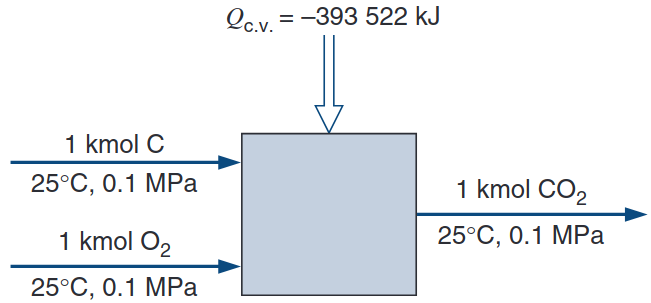
\includegraphics[scale=0.38]{images/comb}
\caption[Ejemplo de proceso de combustión]{Ejemplo de proceso de combustión.\cite{bib:vanwylen}}
\label{fig:comb}
\end{center}
\end{figure}
\begin{equation*}
Q_{c.v.} + H_R = H_P
\end{equation*}

\par Donde los subíndices R y P se refieren a los reactivos y productos, respectivamente. Es conveniente escribir los términos de entalpía como sumas para tal proceso en la forma:
\begin{equation*}
H_R + \sum_R n_i \bar h_i ; \quad H_P + \sum_P n_i \bar h_i
\end{equation*}

\par Donde las sumatorias se refieren, respectivamente, a todos los reactivos y a todos los productos.
\par Por lo tanto, una medida de la transferencia de calor nos daría la diferencia entre la entalpía de los productos y los reactivos, donde cada uno se encuentra en la condición de estado de referencia. Sin embargo, suponga que asignamos el valor de cero a la entalpía de todos los elementos en el estado de referencia. En este caso, la entalpía de los reactivos es cero, y
\begin{equation*}
Q_{c.v.} = H_P = -393,522 kJ/kmol
\end{equation*}

\par La entalpía del \ac{co2} del gas ideal (hipotético) a 25ºC, 0,1 MPa de presión (con referencia a esta base arbitraria en la que la entalpía de los elementos se elige igual a cero) se denomina entalpía de formación. Designamos esto con el símbolo \=h$_f$. Así, para el \ac{co2}
\begin{equation*}
\bar h^0_{f CO_2} = -393,522 kJ/kmol
\end{equation*}
\par La entalpía del \ac{co2} en cualquier otro estado, relativa a esta base en la que la entalpía de los elementos es cero, se encontraría sumando el cambio de entalpía entre el gas ideal a 25ºC, 0,1 MPa y el estado dado a la entalpía de formación. Es decir, la entalpía a cualquier temperatura y presión, h$_{T, P}$, es
\begin{equation*}
\bar h_{T,P} = (\bar h^0_{f})_{298,0.1MPa} + (\Delta \bar h)_{298,0.1MPa \rightarrow T,P}
\end{equation*}
\par Donde el término $(\Delta \bar h)_{298,0.1MPa \rightarrow T,P}$ representa la diferencia de entalpía entre cualquier estado dado y la entalpía del gas ideal a 298.15 K, 0.1 MPa. El procedimiento que se ha demostrado para el \ac{co2} se puede aplicar a cualquier compuesto.

\subsubsection{Entalpía y energia interna de combustion; Valor de calentamiento}

\par La entalpía de combustión, h$_{RP}$, se define como la diferencia entre la entalpía de los productos y la entalpía de los reactivos con combustión completa evaluada a una temperatura y presión dadas. Eso es,
\begin{equation}
\begin{gathered}
\bar h_{RP} = H_P - H_R \\
\bar h_{RP} = \sum_P n_e(\bar h^0_f + \Delta \bar h)_e - \sum_R n_i(\bar h^0_f + \Delta \bar h)_i
\end{gathered}
\end{equation}

\par El parámetro habitual para expresar la entalpía de combustión es una unidad de masa de combustible, como un kilogramo $(h_{RP})$ o un kilomol $(\bar h_{RP})$ de combustible.

Como la entalpía de formación es fija, podemos separar los términos como:
\begin{equation*}
    H = H^0 + \Delta H
\end{equation*}
\par Dónde
\begin{equation*}
    H^0_{R} = \sum_R n_i \bar h^0_{fi} ; \quad H^0_{R} = \sum_R n_i \Delta \bar h_{i}
\end{equation*}
\par Y
\begin{equation*}
    H^0_{P} = \sum_P n_i \bar h^0_{fi} ; \quad H^0_{P} = \sum_P n_i \Delta \bar h_{i}
\end{equation*}
\par Ahora la diferencia de entalpías se escribe
\begin{gather*}
    H_P - H_R = H^0_P - H^0_R + \Delta H_P - \Delta H_R \\
    \quad \quad = H^0_{RP} + \Delta H_P - \Delta H_R
\end{gather*}

\par Mostrando explícitamente la entalpía de combustión de referencia, $H^0_{RP}$, y los dos términos de partida $\Delta H_{P}$ y $\Delta H_{R}$. Los últimos dos términos para los productos y reactivos son distintos de cero si existen en un estado distinto al estado de referencia.
\par Los valores tabulados de la entalpía de combustión de los combustibles suelen darse para una temperatura de 25ºC y una presión de 0.1 MPa. La entalpía de combustión para varios combustibles de hidrocarburos a esta temperatura y presión, que designamos $H^0_{RP}$, fueron obtenidos de las tablas de Borgnakke y Sonntag\cite{bib:vanwylen}.
\par La energía interna de combustión se define de manera similar.
\begin{equation}
\begin{gathered}
    U_{RP} = U_{P} - U_{R} \quad\quad\quad\quad\quad
    \quad\quad\quad\quad\quad\quad\quad\quad\quad\quad\quad\quad\quad\quad\\
    = \sum_P n_e (\bar h^0_{f} + \Delta \bar h - P\bar v)_{e} - \sum_R n_i (\bar h^0_{f} + \Delta \bar h - P\bar v)_{e}
\end{gathered}
\end{equation}
\par Cuando todos los componentes gaseosos se pueden considerar como gases ideales, y el volumen de los componentes líquidos y sólidos es insignificante en comparación con el valor de los componentes gaseosos, esta relación para $\bar u_{RP}$ se reduce a
\begin{equation}
        U_{RP} = H_{RP} - \bar RT (n_{productos gaseosos} - n_{reactivos gaseosos})
\end{equation}
\par Con frecuencia se utiliza el término poder calorífico (PC) o calor de reacción. Esto representa el calor transferido desde la cámara durante la combustión o reacción a temperatura constante. En el caso de un proceso de presión constante o de flujo constante, deducimos de la ecuación de la energía que es igual al negativo de la entalpía de combustión. Por esta razón, esta transferencia de calor a veces se denomina poder calorífico a presión constante para los procesos de combustión.
\par En el caso de un proceso a volumen constante, la transferencia de calor es igual al negativo de la energía interna de combustión. Esto a veces se designa como valor calorífico a volumen constante en el caso de la combustión.
\par Cuando se usa el término poder calorífico, se usan los términos poder calorífico superior e inferior (groso y neto). El poder calorífico superior (gross calorific value GCV) es la transferencia de calor con agua líquida en los productos, y el poder calorífico inferior (net calorific value NCV) es la transferencia de calor con agua vaporizada en los productos.
\par La ecuación de energía para un flujo constante puede ahora ser escrita como:
\begin{equation}
\label{eq:pc}
\begin{gathered}
    W_{c.v.} - Q_{c.v.} = H_R - H_P \quad\quad\quad\quad\quad\quad\quad
    \quad\quad\quad\quad\quad\quad\quad\quad\\
     = \bar H^0_{RP} + \Delta H_R - \Delta H_P \quad\quad\quad\quad\quad\\
     = PC * M_{combustible} + \Delta H_R - \Delta H_P
\end{gathered}
\end{equation}
\par Si los reactivos y los productos entran y salen en las condiciones de referencia, la energía neta que sale ($W_{c.v.} - Q_{c.v.}$) es igual al poder calorífico. Para situaciones en las que los reactivos se precalientan ($\Delta H_R > 0$), la salida de energía neta es correspondientemente mayor, y si los productos salen a una temperatura elevada, $\Delta H_P > 0$, que es lo típico, la salida de energía neta se reduce. Se debe tener cuidado de evaluar todos los términos con la misma escala que la base de masa o mol.

\subsubsection{Temperatura de llama adiabática}
\par En muchas aplicaciones de combustión, la temperatura máxima es importante y la razón varía. Para un motor térmico, una temperatura alta aumenta la eficiencia; para un incinerador o un oxidante térmico, la temperatura máxima garantiza la destrucción de gases o partículas nocivas. Sin embargo, la alta temperatura provoca la formación de varias formas de óxido nítrico, un contaminante que es difícil de eliminar, y ejerce presión sobre todos los materiales expuestos a los productos. La energía en un flujo constante de productos se encuentra a partir de la ecuación de energía, Ec. \ref{eq:pc}, como
\begin{equation}
\begin{gathered}
    \Delta H_P = PC * M_{combustible} + \Delta H_R + W_{c.v.} - Q_{c.v.}
\end{gathered}
\end{equation}
\par Entonces, para un proceso de combustión dado sin trabajo ni transferencia de calor, los dos primeros términos definen la entalpía del producto, y la temperatura del producto se denomina temperatura de llama adiabática. La temperatura depende entonces del estado de los reactivos y de la composición de los productos, por lo que la única temperatura de llama adiabática bien definida ocurre si los reactivos se suministran a la temperatura de referencia ($\Delta H_R$ = 0) y la combustión es completa, de modo que el se conoce la composición del producto.\cite{bib:vanwylen}
\par Para un combustible dado y una presión y temperatura dadas de los reactivos, la temperatura de llama adiabática máxima que se puede lograr es con una mezcla estequiométrica. La temperatura de la llama adiabática se puede controlar mediante la cantidad de exceso de aire que se utiliza. Esto es importante, por ejemplo, en turbinas de gas, donde la temperatura máxima permisible está determinada por consideraciones metalúrgicas en la turbina y es esencial un control estricto de la temperatura de los productos.

\subsection{Balance global}
\par Con los aspectos anteriormente definidos se puede plantear un balance de energía global, usando el horno como volumen de control, ec. \ref{eq:balance-global}, donde se aprecia la distribución del calor generado en la combustión. Ver la Figura \ref{fig:balance-energic}.

\begin{figure}[hbt]
\begin{center}
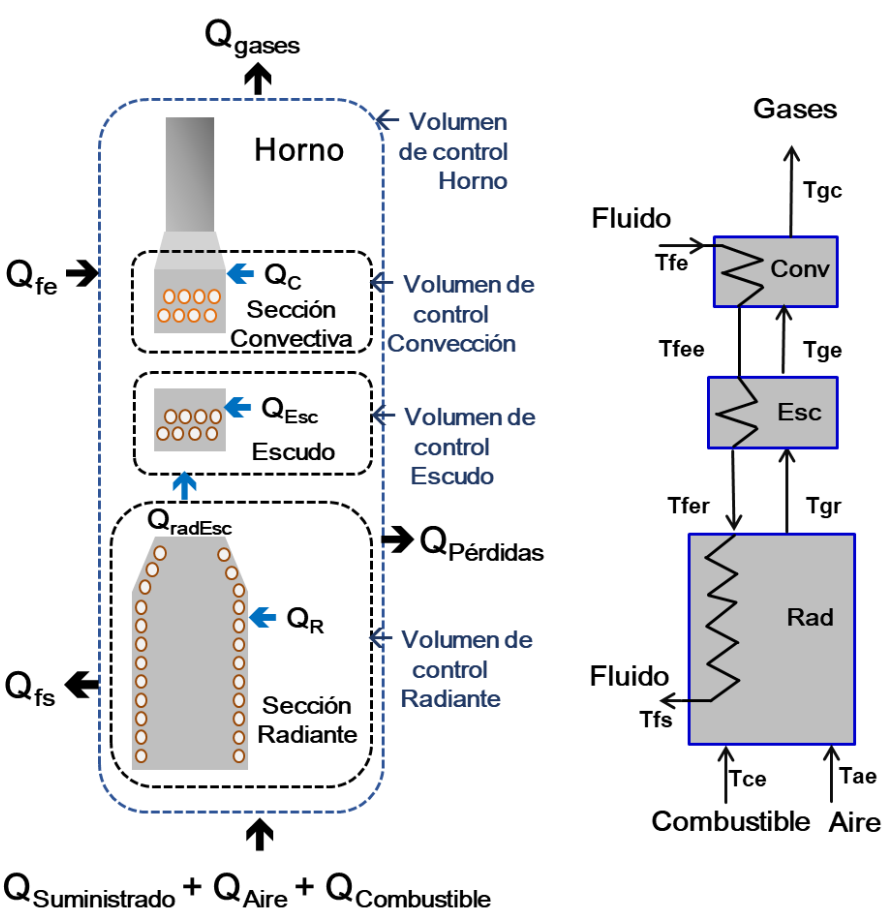
\includegraphics[scale=0.38]{images/balance-energic}
\caption[Balance de energía del horno]{Balance global de energía en el horno y similitud con intercambiador de tres etapas.}
\label{fig:balance-energic}
\end{center}
\end{figure}

\begin{equation}
    \label{eq:balance-global}
    \begin{gathered}
    Q_{entrada} = Q_{salida}\\
    Q_{suministrado} + Q_{aire} + Q_{combustible} + Q_{f_{entrada}} = 
    Q_{gases} + Q_{f_{salida}} + Q_{perdidas}
    \end{gathered}
\end{equation}

donde:\\
$Q_{suministrado} = NCV * m_{combustible}$\\
$Q_{perdidas} = Calor perdido por falta de hermeticidad$\\
$Q_{otros compuestos} = m_{otros compuestos} * Cp_{otros compuestos}(T) * \Delta T$

\section{Zonas y balances de energía en el horno}

\par El horno puede ser dividido en zonas o secciones para simplificar los cálculos, como se pudo apreciar en la sección de tipos de horno, el arreglo mecánico puede variar pero para fines de este análisis se ha dividido el horno en tres zonas o volúmenes de control: radiativa, escudo y convectiva. El volumen de control radiativo corresponde a la sección radiante (o también llamada de radiación) del horno, y los volúmenes de control escudo y convectivo forman parte de una misma sección del horno, la sección convectiva. La división de la sección convectiva es debida a que las dos zonas presentan diferencias en los mecanismos de transferencia de calor, así, los tubos de la zona escudo reciben radiación luminosa directa de la llama,  la cual no está presente en la zona convectiva. La zona escudo está formada por las dos o tres primeras filas de tubos de la sección convectiva y son tubos lisos, mientras que la zona convectiva está formada generalmente por tubos con aletas. En ambas zonas está presenta la radiación del gas y la reflectada de las paredes de la sección hacia los tubos. Esta radiación, de baja longitud de onda, deja de ser significativa por debajo de los 550 C (1000 F).
 
\par Conociendo que la energía transferida al fluido de proceso es igual a

\begin{equation}
    \begin{gathered}
    Q_{fs} - Q_{fe} = Q_{RAD} + Q_{ESC} + Q_{CONV}\\
               	    = m_f * C_p * (T_{fs} - T_{fe})
    \end{gathered}
\end{equation}

\par Donde $Q_{RAD}, Q_{ESC}, Q_{CONV}$ son el calor que transfiere el gas de combustión al fluido en las zonas radiante, de escudo y convectiva respectivamente y que corresponde al servicio (duty) del horno, substituyendo en ecuación \ref{eq:balance-global}.

\begin{equation}
    Q_{suministrado} + Q_{aire} + Q_{combustible} = Q_{RAD} + Q_{ESC} + Q_{CONV} + Q_{perdidas} + Q_{gases}
\end{equation}

\par La incógnita se reduce a cuantificar $Q_{RAD}, Q_{ESC}, Q_{CONV}, Q_{perdidas}$ y la temperatura de salida de los gases con el objetivo de:
\begin{enumerate}
    \item Dimensionar el horno para un determinado servicio o duty, y calcular la cantidad de combustible requerido, $Q_{suministrado}$.
    \item Calcular el comportamiento del horno ante variaciones de las condiciones operacionales, tales como, cambios en la composición de combustible, en la relación aire-combustible, el flujo del fluido de proceso, el requerimiento de temperatura de salida del fluido, etc.
\end{enumerate}

\subsection{Zona Radiante}
\par Es donde los tubos que trasportan el fluido de proceso reciben radiación directa desde la llama del quemador y las paredes refractarias. En esta parte la transmisión de calor es por radiación en un 80\% aproximadamente, y un 20\% por convección de la circulación de gases calientes alrededor de los tubos.

\par El análisis descrito a continuación está basado en el modelo presentado inicialmente por (Lobo \& Evans)\cite{bib:rad} y parte de la suposición de un mezclado ideal de los gases producto de la combustión en la sección radiante lo cual implica, en consecuencia, una temperatura uniforme del gas en todo el volumen de la sección radiante, denominada \ac{tg}, la cual será la temperatura efectiva de transferencia de calor entre los gases de combustión y la superficie de los tubos y será igualmente la \ac{tgr} hacia el escudo de tubos.

\par Realizando el balance de energía en el volumen de control de la sección radiante resulta:

\begin{equation}
    \label{eq:rad}
    Q_{suministrado} + Q_{aire} + Q_{combustible} = 
    Q_{RAD} + Q_{radEsc} + Q_{CONV} + Q_{perdidas} + Q_{gases}
\end{equation}

\par En la zona radiante se transfiere calor al fluido por dos mecanismos, mediante radiación directa y por convección entre los gases producto de la combustión y el fluido,

\begin{equation}
    \label{eq:rad-fluid}
    Q_{RAD} = Q_{rad} + Q_{conv} = m_f * C_{p_f} * (T_{fs} - T_{fer})
\end{equation}

\par Donde $Q_{rad}, Q_{conv}$ son el calor que se transfiere al fluido en la sección radiante por radiación y por convección, y $Q_{radEsc}$ es el calor por radiación que se transfiere a los tubos del escudo desde la zona radiante.

\par Usando las siguientes ecuaciones de transferencia de calor:
\begin{equation}
    Q_{rad} = \sigma * ( \alpha * A_{cp} )_{R} * F * ( T_{g}^{4} - T_{w}^{4} )
\end{equation}
$\sigma$ = Constante de Stefan-Boltzman.\\
$\alpha$ = Factor de efectividad relativa del banco de tubos.\\
$A_{cp}$ = Área del plano frontal a la llama del banco de tubos.\\
F = Factor de transferencia radiante.\\
$T_g$ = Temperatura efectiva del gas en la zona radiante (°R o K)\\
$T_w$ = Temperatura promedio de la pared del tubo, (°R o K)

\begin{gather}
    Q_{conv} = h_{conv} * A_t * (T_g - T_w)\\
    Q_{radEsc} = \sigma * ( \alpha * A_{cp} )_{Esc} * F * ( T_{g}^{4} - T_{w}^{4} )
\end{gather}

\par Si se considera que las pérdidas por las paredes del horno equivalen al 1.5\% del calor suministrado (entre 1,5 y 5.0) los calores resultan en:
\begin{gather}
    Q_{suministrado} = NCV * m_{combustible}\\
    Q_{perdidas} = 0.015 * NCV * m_{combustible}\\
    Q_{aire} = m_{aire} * C_{p_A} * (T_A - T_{Ref})\\
    Q_{combustible} = m_{combustible} * C_{p_C} * (T_C - T_{Ref})\\
    Q_{gases} = m_{gases} * C_{p_g} * (T_g - T_{Ref})
\end{gather}

\par Donde $T_{Ref}$ es la temperatura de referencia utilizada para calcular las propiedades termodinámicas (condiciones estándar de presión y temperatura).

\begin{equation}
    m_{gases} = m_{combustible} * AC_{masa} + m_{combustible} = 
    m_{combustible} (1 + AC_{masa})
\end{equation}

Substituyendo  en las ecuaciones (\ref{eq:rad}) y (\ref{eq:rad-fluid}) se obtiene:

\begin{equation}\label{eq:rad-tgr}
\begin{gathered}
    m_C*NCV +m_A*C_{p_A}*(T_A -T_{Ref}) + m_C*C_{p_C}*(T_C -T_{Ref}) = \\
    m_C*(1 +AC_{masa})*C_{p_G}*(T_g -T_{Ref}) + \\
    \sigma *(\alpha *A_{cp})_{Esc}*F*(T_g^4-T_w^4) + \\
    \sigma *(\alpha *A_{cp})_R F (Tg4 - Tw4) + \\
    h_{conv}*A_t*(T_g -T_w) + \\
    0.015*m_C*NCV
\end{gathered}
\end{equation}
\begin{equation}
\label{eq:rad-comp}
Q_R = 
\sigma * (\alpha * A_{cp})_R *F *(T_g^4 -T_w^4) +h_{conv} *A_t *(T_g -T_w)
= m_f * C_{p_f} * (T_{fs} - T_{fer})
\end{equation}
\par La ecuación (\ref{eq:rad-tgr}) permite calcular la \ac{tgr}, o el flujo másico de combustible requerido, $m_C$, mediante un proceso de ensayo-error o en su defecto, utilizando un algoritmo de cálculo numérico (p. ej., el método usado para este desarrollo fue Newton Raphson). La ecuación (\ref{eq:rad-comp}) permite calcular la  temperatura efectiva de llama Tgr a partir de un estimado del calor transferido al fluido en la zona radiante ($Duty_{rad}$).

\subsubsection{Temperatura de pared (Tw)}
\par La temperatura de pared puede ser calculada a partir de la ecuación de transferencia de calor entre el fluido y la pared externa del tubo:
\begin{equation*}
    q_{rad} = Q_R / A_o
\end{equation*}

donde $q_{rad}$ es el flujo de calor por unidad de área exterior del tubo (densidad de flujo de calor) en la zona radiante.
\begin{gather*}
q_{rad} = \frac{(Q_{rad} + Q_{conv})}{A_o} = (T_w - T_b) / (A_t *\Sigma R) \\
\Sigma R = R_{conv} + R_{fi} + R_t
\end{gather*}

\par Que corresponden a la resistencia convectiva interna, el factor de ensuciamiento y la resistencia conductiva de la pared del tubo. Resolviendo por $T_W$
\begin{equation}
\label{eq:tw}
T_W = q_{rad} *(d_o/d_i) *[ R_{fi} + 1/h_i + d_i*ln(d_o/d_i)/(2*k_w) ] +T_b
\end{equation}

\par Donde,\\
$T_b$ es la temperatura de mezcla del fluido $(T_{fs} + T_{fer})/2$. \\
$k_w$ es la conductividad térmica del tubo. \\
$h_i$ es el coeficiente interno de transferencia de calor. \\
$R_{fi}$ es el factor de ensuciamiento interno del tubo. \\

\par Para resolver la ecuación (\ref{eq:tw}) se necesita calcular la temperatura de entrada del fluido a la zona radiante, $T_{fer}$ a partir del estimado hecho de $Q_R$. 

\subsubsection{Coeficiente interno de transferencia de calor (coeficiente de película del fluido)}

\par El coeficiente interno de transferencia de calor es calculado para líquidos por la ampliamente usada ecuación
\begin{equation}
\label{eq:hi}
 h_i = 0.023 * \frac{k_f}{d_i} *Re^{0.8} *Pr^{1/3} *(\mu_b /\mu_w )^{0.14}
\end{equation}
\par Donde,\\
$\mu_b$ y $\mu_w$ son las viscosidades del fluido de proceso a $T_b$ y $T_w$. \\
Re, es el número de Reynolds evaluado a la temperatura $T_b$. \\
Re = $(\rho v d_i / \mu)_b = (G *d_i / \mu)_b$. \\
G, es el flujo másico por unidad de área. \\
Pr, es el número de Prandtl del fluido de proceso. \\
Pr = $(\mu C_p / k)_f$ evaluado a $T_b$.

\subsubsection{Coeficiente convectivo de la zona radiante}
\par El coeficiente convectivo de la parte exterior de los tubos en la zona convectiva, para un horno tipo cabina con tubos en la pared ha sido estimado en
\begin{equation}
h_{conv} = 1.5  BTU/(hr ft^2 F) \approx 8.5 W/(m^2 C)
\end{equation}
\par Con esta última ecuación quedan definidos todos los términos de las ecuaciones (\ref{eq:rad-tgr}) y (\ref{eq:rad-comp}).

\subsubsection{Factor de eficiencia del banco de tubos ($\alpha$)}
\par Factor de eficiencia, $\alpha$, debido a que el banco de tubos no absorbe todo el calor radiado al área de plano equivalente, un factor de eficiencia de absorción puede ser usado para corregir esta área y dependerá del arreglo de tubos. El factor de eficiencia relativa se describe bajo las siguientes curvas:
\par Para una fila de tubos simple frente a la pared refractaria, usar (Total One Row). Para dos filas de tubos frente a la pared refractaria, usar (Total Two Rows). Para hornos de doble llama, usar (Direct OneRow). Ver la Figura \ref{fig:alpha}.

\begin{figure}[hbt]
\begin{center}
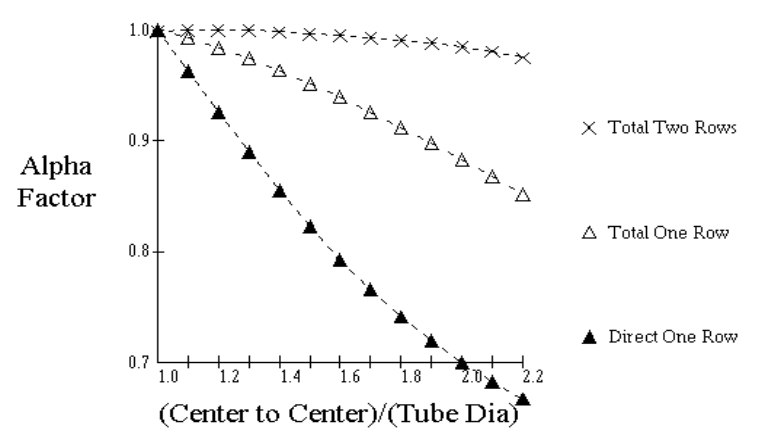
\includegraphics[scale=0.45]{images/alpha}
\caption[Eficiencia de absorción para banco de tubos]{Eficiencia de absorción para banco de tubos.}
\label{fig:alpha}
\end{center}
\end{figure}

\subsubsection{Área del plano equivalente que reemplaza el área de los tubos (Acp radiante)}
\par Las superficies normales de absorción de calor en un horno consisten en una serie de tubos paralelos. En el caso de un diseño de hornos donde los tubos se reciben la llama desde un solo lado, los tubos normalmente se colocan frente a una pared refractaria. Parte de la radiación del gas caliente incide directamente en los tubos, mientras que el resto pasa a través de las hileras y se irradia de regreso a la cámara, donde parte es absorbida por los tubos al ser refractada en las paredes. En el caso de tubos expuestos desde ambos lados, por ejemplo, cuando los tubos están colocados en el centro de la cámara, los tubos absorben la radiación directa desde ambos lados. Expresar el área del tubo como un área plana equivalente simplifica este cálculo. El área de plano equivalente calculada es el área de un plano a través de las líneas centrales del tubo, ya sea que estén en un plano curvo, como en un patrón cilíndrico o en una fila de lado a lado. Para la mayoría de los paneles de tubos, el ancho sería igual al espacio centro/centro de los tubos multiplicado por el número de tubos. La longitud efectiva es la longitud del tubo expuesto a la radiación. En el caso de tubos que penetran en una placa tubular, es la longitud entre placas tubulares. Pero para los tubos con las curvas de retorno dentro de la cámara de combustión, la longitud puede tomarse como la distancia desde la línea central del retorno en un extremo hasta la línea central del retorno en el otro extremo.
\par Para una cámara de combustión con los tubos hacia abajo en el centro, u otro patrón que resulte en que los tubos se disparen desde ambos lados, el área de plano equivalente sería el doble del área proyectada.
\par Para llama de un solo lado:
\begin{equation}
Acp = N_{tubo} * S_{tubo} * L_{tubo}
\end{equation}
\par Para llama de ambos lados:
\begin{equation*}
Acp = N_{tubo} * S_{tubo} * L_{tubo} * 2
\end{equation*}
\par Donde, \\
$N_{tubo}$ = Número de tubos. \\
$S_{tubo}$ = Espaciado de tubos. \\
$L_{tubo}$ = Largo efectivo del tubo.

\subsubsection{Factor global de transferencia radiante (F)}
\par Debido a que el gas de combustión en el horno es un mal medio de radiación, la ecuación debe ser corregida usando un factor de transferencia radiante dependiente de la emisividad del gas y la relación del área refractaria de plano equivalente. Como el calor de radiación es reflejado de regreso al horno, por refracción, un horno con mayor relación de de superficie refractaria con respecto a la superficie de los tubos, absorberá mas calor. Como los tubos no absorben perfectamente el calor, las curvas esta basadas en superficies de tubos con absorción de 0.9. Un valor considerado como típico para superficies de metales oxidados. El factor de transferencia radiante final puede ser tomado de la siguiente curva (Figura \ref{fig:f}) ofrecida por Mekler \& Fairall\cite{bib:mekler}.
\begin{figure}[hbt]
\begin{center}
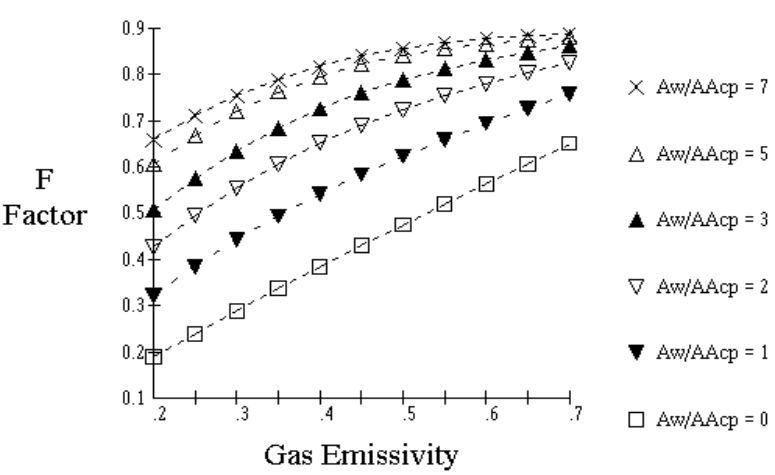
\includegraphics[scale=0.45]{images/f}
\caption[Factor de transferencia radiante, F]{Factor de transferencia radiante, F.\cite{bib:mekler}}
\label{fig:f}
\end{center}
\end{figure}
\par Donde $Aw$/$\alpha$Acp es calculada con la ecuación \ref{eq:aw-acp}. El área de plano equivalente efectiva, $\alpha$Acp, es el producto del factor de efectividad y del área de plano equivalente como se describió anteriormente. Área refractaria efectiva se calcula con:
\begin{equation}
Aw = Ar - \alpha Acp
\end{equation}
\par El área refractaria total, Ar, es el total del área refractaria expuesta a la sección radiante del horno. Cuando hay sección de escudo, que recibe radiación directa, el $\alpha$Acp para la sección radiante y para la sección de escudo se calculan de forma independiente y luego son sumados para calcular el factor de transferencia radiante.
\par La ecuación para $Aw$ se convierte en:
\begin{equation}
Aw = Ar - ((\alpha Acp)_{rad} + (\alpha Acp)_{esc})   
\end{equation}
\par Para finalmente:
\begin{equation}
\label{eq:aw-acp}
Aw/\alpha Acp = \frac{Aw}{(\alpha Acp)_{rad} + (\alpha Acp)_{esc}}
\end{equation}
\subsubsection{Emisividad de gases de combustión}
\par La emisividad de un gas puede ser descrita por la curva presentada por Lobo y Evans\cite{bib:rad}, la temperatura de pared tiene solo un efecto menor. Por lo tanto, la emisividad puede ser correlacionada como una función de la suma de las presiones parciales del vapor de agua y el dióxido de carbono (P), multiplicada por la longitud media del haz radiante (L), (PL, ec. \ref{eq:pl}) producida y la temperatura del gas de combustión, Tg. Variaciones en la temperatura de pared entre 600ªF y 1200 ªF causan una desviación menor al 1\% de estas curvas.

\begin{figure}[hbt]
\begin{center}
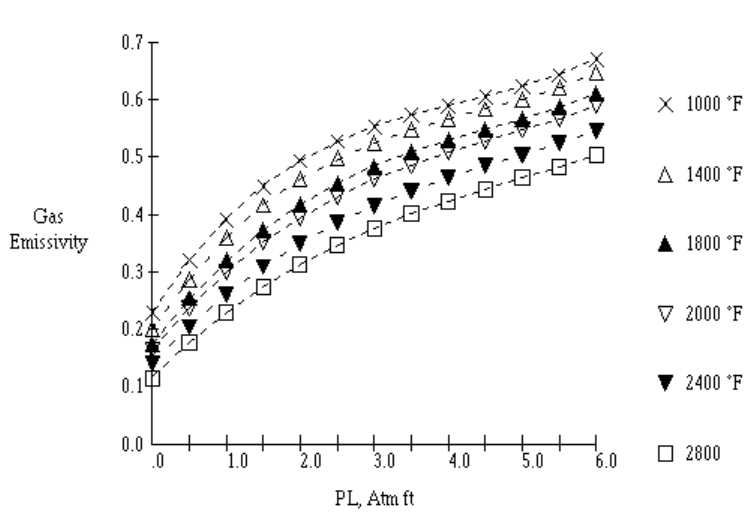
\includegraphics[scale=0.45]{images/emiss}
\caption[Emisividad del gas]{Emisividad del gas.\cite{bib:mekler}}
\label{fig:emiss}
\end{center}
\end{figure}
\begin{equation}
\label{eq:pl}
PL = (PH_2O + PCO_2) * MBL
\end{equation}
\par Donde $PH_2O$ y $PCO_2$ son las presiones parciales del \ac{h2o} y \ac{co2} en el gas, y MBL en pies obtenido de la tabla \ref{tbl:mbl}.

\subsubsection{\ac{mbl}}
\par Para el cálculo de la \ac{mbl}, la distribución de los tubos debe ser tomada en cuenta. Si el horno es de forma rectangular con tubos en el centro, la \ac{mbl} será la mitad del área rectangular del horno. Longitudes del haz radiante para otras configuraciones, como un horno cilíndrico con una disposición de tubos octagonal o tubos cruzados, deberá ser calculada con esas consideraciones.
\par La \ac{mbl} para hornos puede ser tomada, de acuerdo a Wimpress\cite{bib:wimpress} como se muestra en la Tabla \ref{tbl:mbl}.:
\begin{table}
\caption[Calculo del MBL]{Cálculo del MBL con dependencia de las dimensiones de la cámara de combustión}
\label{tbl:mbl}
    \centering
    \begin{tabular}{c|c}
        Relación de dimensión  & Longitud media del haz radiante \\
        \hline
        1-1-1 a 1-1-3   & \multirow{2}{10em}{2/3 * (Vol. horno)$^{1/3}$} \\
        1-2-1 a 1-2-4   & \\
        \hline
        1-1-4 a 1-1-inf & 1 * Menor dimensión \\
        \hline
        1-2-5 a 1-2-inf   & 1.3 * Menor dimensión \\
        \hline
        1-3-3 a 1-inf-inf & 1.8 * Menor dimensión \\
        \hline
        \multicolumn{2}{c}{Para hornos cilíndricos verticales} \\
        \hline
        Largo/Diámetro $<$ 2  & (($\frac{L}{D}$-1)*0.33 + 0.67)*D\\
        \hline
        Largo/Diámetro $\geq$ 2 & Diámetro\\
    \end{tabular}
    \caption{MBL para hornos rectangulares}
    \label{tbl:mbl}
\end{table}

\subsection{Zona Escudo}
\par Esta zona contiene las primeras filas de tubos del área de convección que "protegen" (\textit{shield}) el resto de la zona de convección, en ella los tubos no tienen aletas y reciben la misma cantidad de calor por ambos mecanismos.

\par Según  han reportado  Mekler \& Fairall\cite{bib:mekler}  la radiación luminosa desde la sección radiante a los tubos de la zona escudo, $Q_{radEsc}$ puede ser repartida un 76.92\% en la primera fila y el 23.08\% restante en la segunda fila. Esta aproximación conjuntamente con la distribución circular del flujo de calor es usada para calcular la temperatura máxima de pared en los tubos de la zona de escudo.
\par Realizando un balance de energía en la zona de los tubos de escudo
\begin{equation}
\label{eq:esc}
Q_{entradaEsc} = Q_{fe} + Q_{gas-e} + Q_{radEsc} = 
Q_{fs} + Q_{gas-s} = Q_{salidaEsc}
\end{equation}
\par Donde $Q_{radEsc}$ es el calor por radiación que escapa desde la zona radiante hacia el escudo de tubos y que ya ha sido calculado al determinar la temperatura efectiva de radiación Tg. La temperatura de entrada del gas a la zona de escudo Tgr es igual a la temperatura efectiva Tg, lo cual se infiere de haber supuesto una temperatura de mezcla ideal de los gases en la sección radiante. $Tgr = Tg$
\par Rearreglando la ecuación \ref{eq:esc}, se obtiene:
\begin{equation*}
Q_{fs} - Q_{fe} = Q_{gas-e} - Q_{gas-s} + Q_{radEsc} = Q_{Esc}
\end{equation*}
\par Donde,
\begin{equation}
\label{eq:qesc}
m_{f} *C_{p_f} *(T_{fer} - T_{fee}) = 
m_{g} *C_{p_g} *(T_{gr}  - T_{ge}) + Q_{radEsc} = Q_{Esc}
\end{equation}
\begin{equation}
Q_{radEsc} = \sigma *(\alpha *A_{cp} )_{Esc} *F *(T_{gr}^4 -T_w^4)
\end{equation}

\par Para los gases el cambio de entalpía dentro de zona del escudo se debe a la transferencia de calor hacia los tubos.
\begin{equation}
\label{eq:qesc-lmtd}
m_{g} *C_{p_g} *(T_{gr} -T_{ge}) = Uo *Ao *LMTD
\end{equation}

\par Donde LMTD es la Diferencia de Temperatura Media Logarítmica entre el gas de combustión y el fluido del proceso, expresada por:
\begin{equation}
\label{eq:lmtd}
   LMTD = \frac{(T_{gr}-T_{fer}) - (T_{ge}-T_{fee})}
   {ln[(T_{gr}-T_{fer}) /(T_{ge}-T_{fee})]}
\end{equation}
Sustituyendo (\ref{eq:qesc-lmtd}) en (\ref{eq:qesc})
\begin{equation}
\label{eq:tesc}
  Q_{Esc} = m_{f} *C_{p_f} *(T_{fer} - T_{fee}) = Uo *Ao *LMTD + Q_{radEsc}
\end{equation}

\subsubsection{Coeficiente Global de Transferencia de Calor en el Escudo}
\par Generalmente el escudo de tubos está formado por dos o tres filas de tubos lisos (sin aletas) pero formando parte del banco de tubos de la sección superior del horno que incluye otra zona de tubos aletados, para un banco de tubos lisos el coeficiente global de transferencia de calor viene dado por la ecuación:
\begin{gather*}
\label{}
Uo  = 1 / \Sigma R \\
\Sigma R = R_o + R_t + R_i
\end{gather*}

\par Donde $R_o, R_t, R_i$ son la resistencia externa de la pared del tubo, la resistencia interna del tubo y el factor de ensuciamiento interno respectivamente.
\par Sustituyendo:
\begin{equation}
\label{}
\Sigma R = \frac{1}{h_o} +\frac{d_o*ln(d_o/d_i)}{2*k_t} +\frac{A_o}{A_i*h_i} +R_{fi}
\end{equation}
\begin{equation}
\label{}
m_{g} *C_{p_g} *(T_{gr} - T_{ge}) = \frac{Ao *LMTD}
{\frac{1}{h_o} +\frac{d_o*ln(d_o/d_i)}{2*k_t} +\frac{d_o}{d_i*h_i} +\frac{d_o}{d_i}R_{fi}}
\end{equation}

\par Donde el coeficiente interno de película se calcula como en el caso de los tubos de la sección radiante mediante la ecuación \ref{eq:hi}:
\par El coeficiente externo $h_o$ puede ser expresado como la sumatoria de las resistencias externas como:
\begin{equation}
\label{eq:ho}
h_o = 1/(\frac{1}{h_c + h_{re}} + R_{fo})
\end{equation}
\par Donde \\
$h_c$ es el coeficiente de película externo.\\
$h_r$ es el coeficiente efectivo de radiación hacia la pared del tubo.\\
$R_{fo}$ es el factor de ensuciamiento externo.\\

\par El coeficiente de película exterior para un banco de tubos lisos colocados triangularmente (tresbolillo) puede ser calculado por:
\begin{equation}
\label{eq:hc}
\begin{gathered}
h_c = 0.33 * \frac{k_{gb}}{d_o} *Pr_{gb}^{1/3} *Re_{gb}^{0.6}\\
h_c = 0.33 * \frac{k_{gb}}{d_o} *Pr_{gb}^{1/3} *(\frac{d_o*G_n}{\mu_{gb}})^{0.6}
\end{gathered}
\end{equation}
$G_n$ es la velocidad másica basada en el área libre para el flujo de gas, es decir, el espacio entre los tubos por el largo del horno.

\par El coeficiente efectivo de radiación se refiere al calor por radiación que transfiere el gas de combustión más el calor reradiado de las paredes de la zona de escudo a la pared de los tubos. Como aproximación el coeficiente de radiación para la zona de escudo y convectiva puede ser obtenido de la siguiente ecuación empírica:
\begin{equation}
\label{eq:hr}
h_r = 0.092*T_g - 34  
\end{equation}
\par Donde Tg es la temperatura del gas en °K y $h_r$ viene expresado en kJ/m$^2$h°K

\par Otro método para el cálculo de $h_{re}$ se tratará más adelante, conjuntamente con el de la zona convectiva.

\subsubsection{Coeficiente efectivo de absorción de radiación. Tubos escudo}
\par Dado que todo el calor dirigido hacia este banco de tubos sale de la sección radiante y es absorbido por los tubos, el factor de efectividad de absorción relativa, $\alpha$, para los tubos de escudo puede tomarse igual a uno.

\subsubsection{Área del plano equivalente que reemplaza el área de los tubos (Acp escudo)}
\par El área de plano equivalente para la sección de escudo es igual al área de plano equivalente de la primera fila de tubos de esta sección.
\begin{equation*}
Acp = N_tubo * S_tubo * L_tubo
\end{equation*}
\par Donde, \\
$N_{tubo}$ = Número de tubos por fila. \\
$S_{tubo}$ = Espaciado de tubos. \\
$L_{tubo}$ = Largo efectivo del tubo.\\
\par Los valores usados para el factor de intercambio, F, temperatura efectiva del gas en la cámara de radiación, Tgr, y temperatura de pared promedio, Tw, son los mismos valores usados en la sección radiante.

\subsection{Zona Convectiva}
\par En esta zona el calor del gas hacia los tubos se transfiere en forma similar al de la zona escudo. En el lado exterior de los tubos se trasfiere calor por radiación y por convección en paralelo, pero en este caso la presencia de las aletas modifica el cálculo de los coeficientes de transferencia de calor.

\par El balance de energía depende de la energía entrando y saliendo del gas y del fluido del proceso resulta en:

\begin{equation}
\label{eq:conv}
Q_{entrada} = Q_{fe} + Q_{gas-e} = Q_{fee} + Q_{gas-s} = Q_{salida}
\end{equation}

\par Rearreglando:
\begin{equation*}
Q_{fee} - Q_{fe} = Q_{gas-e} - Q_{gas-s} = Q_{CONV}
\end{equation*}
\begin{equation}
\label{eq:qconv}
m_{f} *C_{p_f} *(T_{fer} - T_{fee}) = 
m_{g} *C_{p_g} *(T_{ge}  - T_{gc}) = Q_{CONV}
\end{equation}
\par Los valores de $C_{p_f}$ y $C_{p_g}$ son calculados a la temperatura promedio del fluido y del gas.

\subsubsection{Transferencia convectiva, tubos aletados}
\par Las ecuaciones de transferencia de calor para los tubos con aletas son básicamente las mismas que para los tubos lisos hasta que llega al factor $h_e$, donde se introduce un nuevo concepto para explicar la aleta o superficie extendida.

\subsubsection{Coeficiente global de transferencia de calor, Uo}

\begin{equation}
Q_{CONV} = Uo *Ao *LMTD
\end{equation}

\begin{gather*}
\label{}
Uo  = 1 / \Sigma R \\
\Sigma R = R_o + R_t + R_i \\
\Sigma R =  \frac{1}{h_{oe}} 
            +\frac{d_o*ln(d_o/d_i)}{2*k_t} 
            +(\frac{1}{h_i}+R_{fi})*\frac{d_o}{d_i} 
\end{gather*}

\subsubsection{Coeficiente externo efectivo de transferencia de calor, $h_{oe}$}
\par Proveniente de la siguiente ecuación.
\begin{equation*}
h_{oe} = h_o * (E *Afo +Apo) / Ao
\end{equation*}

\par Donde,\\
E = Eficiencia de las aletas\\
Ao = Área de superficie externa total.\\
Afo = Área de superficie externa de aletas. \\
Apo = Área de superficie de tubos. \\

\par Y, $h_o$, coeficiente externo promedio de transferencia de calor: 
\begin{equation*}
h_o = 1/(\frac{1}{h_c+h_r}+R_{fo})
\end{equation*}

\par Donde,\\
$h_r$ = Coeficiente externo de radiación de transferencia de calor.\\
$R_{fo}$ = Resistencia de ensuciamiento externo. \\

\par Y, $h_c$, coeficiente de película externo de transferencia de calor: 
\begin{equation*}
h_c = j *G_n *C_{p_g} *(Pr_g)^{0.67}
\end{equation*}

\par Donde,\\
j = Factor Colburn de transferencia de calor.\\
$G_n$ = Velocidad másica basada en el área libre neta.\\
$Pr_g$ = Número de Prandtl del gas $(\mu*C_p /k)_{gb}$ evaluado a $T_{gb}$.\\
$C_{p_g}$ = Capacidad calorífica del gas.\\
$k_b$ = Conductividad térmica del gas.\\
$\mu_b$ = Viscosidad dinámica del gas.\\

\subsubsection{Factor Colburn de transferencia de calor, j}
\par Dado por la siguiente correlación.
\begin{equation*}
j = C_1 *C_3 *C_5 *(\dfrac{d_f}{d_o})^{0.5} *(\frac{T_b}{T_s})^{0.25}
\end{equation*}

\par Donde, \\
$C_1$ = Corrección del número de Reynolds. \\
$C_3$ = Corrección geométrica. \\
$C_5$ = Corrección no-equilateral y de fila. \\
$d_f$ = Diámetro externo de la aleta. \\
$d_o$ = Diámetro externo del tubo. \\
$T_b$ = Temperatura promedio del gas, K. \\
$T_s$ = Temperatura promedio de aleta, K.\\

\par Corrección del número de Reynolds:
\begin{equation*}
C_1 = 0.25 *Re^{-0.35}
\end{equation*}

\par Corrección geométrica (para aletas sólidas en patrón escalonado):
\begin{equation*}
C_3 = 0.35 +0.65 *e^{-0.25*l_f/s_f}
\end{equation*}
\par Donde, \\
$l_f$ = Altura de aleta. \\
$s_f$ = Espaciado de aleta.\\

\par Corrección no-equilateral y de fila (para tubos aletados en patrón escalonado):
\begin{equation*}
C_5 = 0.7 +(0.70 -0.8 *e^{-0.15 *N_r^2}) *e^{-P_l/P_t}
\end{equation*}
\par Donde, \\
$N_r$ = Numero de tubos por fila. \\
$P_l$ = Paso de tubo longitudinal.\\
$P_t$ = Paso de tubo transversal. \\

\subsubsection{Coeficiente de radiación del gas, $h_r$}
\par Puede ser calculado de las siguientes correlaciones. Este factor se utiliza para calcular el coeficiente global de transferencia de calor para tubos lisos y tubos con aletas. 
Para tubos lisos,
\begin{equation*}
h_r = 2.2 *\gamma_r *PL^{0.50}
\end{equation*}

\par Y para tubos con aletas,
\begin{equation*}
h_r = 2.2 *\gamma_r *PL^{0.50} *(Apo/Ao) *0.75
\end{equation*}

\par Donde,\\
PL tomado de la ecuación \ref{eq:pl}.\\
$\gamma_r$ = Factor de radiación externo.\\
Apo = Área de superficie expuesta de tubos lisos.\\
Ao = Área de superficie externa total. \\

El factor de radiación externo puede ser hallado en las curvas de la figura \ref{fig:gamma}.

\begin{figure}[hbt]
\begin{center}
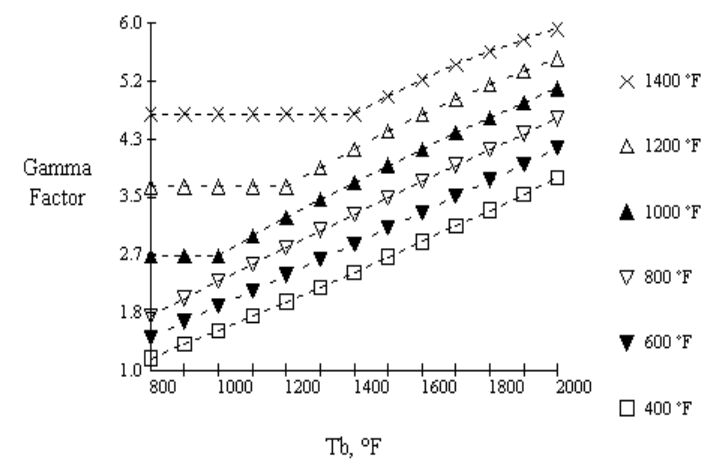
\includegraphics[scale=0.45]{images/gamma}
\caption[Factor de radiación externo]{Factor de radiación externo. Este gráfico requiere de la temperatura promedio del gas y de la temperatura promedio de la superficie del tubo.}
\label{fig:gamma}
\end{center}
\end{figure}